% \section{Social Movements and the Modeling Gap}





% \textcolor{blue}{This tool is needed because conventional energy planning and
% modeling have not yielded a single best course of action to address climate
% change. Indeed, there is no best answer, yet decision-makers employing
% traditional \ac{esom} techniques would lead you to believe so. There are many
% papers identifying nuclear energy as necessary to resolve climate change, and
% others arguing for 100\% renewable energy. \Acp{esom} demonstrate the
% feasibility of using both. How are decision-makers and their constituents
% supposed to choose among apparently equally feasible alternatives? Thus, a
% novel framework for energy modeling is necessary. One that clearly identifies
% trade-offs among conflicting objectives.}



% \begin{enumerate} \item In the absence of corruption (defined as making
%     decisions for personal gain at the expense of fulfilling the duties of a
%     job), policy-makers largely base their decisions on economic merits. \item
%     Why is there a gap between the demonstrated need for a transition away
%     from fossil fuels and the adoption of clean energy? \end{enumerate}



% 8. What do surveys suggest is the reason for opposition to energy projects?
%    \textcolor{red}{\acp{esom} typically model energy transitions at a national
%    or sub-national level, yet siting, permitting, and budgetary decisions are
%    typically made at the local level (subject to regulatory review).}


% \textcolor{orange}{It seems like \ac{osier} could turn into a \ac{pve} tool.
% Previously, I had envisioned users creating their own objectives, or a
% community engagement might start by identifying important objectives to that
% community. That might still be an aspect of the process, and an important one
% for assessing community preferences for different technologies, however later
% iterations of the process, participants may just be given a set of policies to
% rank or choose from. One reason that traditional \acp{esom} do not work with
% the \ac{pve} paradigm, is that total cost cannot be set as a constraint -- it
% is virtually always the thing to be minimized.}

% \noindent\hrulefill

% Addressing ``structural uncertainty'' with \ac{mga} in \acp{esom} is ignorant
% of the significant body of social acceptance research. Social acceptance is an
% essential determinant of the success or failure of an energy project (cite).

% \noindent\hrulefill
\section{Characterizing the Problem of Climate Change}
\label{section:climate-change-risk}
% Questions

% \begin{enumerate}

% \item What are the risks of climate change and failure to respond?

Risk is generally understood as the ``potential for adverse consequences''
\cite{reisinger_concept_2020}. However, due to the complexity of climate change,
the \ac{ipcc} developed a three-tenet framework to discuss risk
\cite{reisinger_concept_2020}: hazard, exposure, and vulnerability.
\textit{Hazards} are mediated by physical features, such as climate and
topography \cite{dorkenoo_critical_2022, simpson_framework_2021}.  Climate
change is already producing more significant hazards, like forest fires, hurricanes,
storms, floods, droughts, and heat waves \cite{reidmiller_fourth_2018,
intergovernmental_panel_on_climate_change_climate_2021, dahl_killer_2019}.
\textit{Exposure} refers to the scale and duration of the subjection of people,
infrastructure, and social wealth to a particular hazard
\cite{simpson_framework_2021,reisinger_concept_2020,li_understanding_2021}.
\textit{Vulnerability} is the ability of a system to cope, recover, and adapt
after exposure to a hazard. Although climate change is a worldwide phenomenon,
vulnerabilities to its hazards are not uniformly distributed. On the contrary, 
the people and communities most likely to be harmed by climate change are already 
harmed by social inequities \cite{islam_climate_2017}. Recent work
from Simpson et al. \cite{simpson_framework_2021} expanded on this definition of
risk by including \textit{responses} to risk as itself a driver of risk. This
framework is illustrated in Figure \ref{fig:risk-framework} using infrastructure risk 
as an instructive example. Considering the
actions taken (or not) in response to climate change is vital for a holistic
understanding of risk because it encompasses benefits and mitigating outcomes,
not just negative, inflammatory ones. Additionally, heterogeneous stakeholders
perceive the costs and benefits of (in)action differently. Therefore,
including response as a driver of risk is essential for making choices more
transparent and actionable within decision-making structures
\cite{simpson_framework_2021}. Responses to climate change risk come in myriad
forms,  and at multiple scales, from individual choices (e.g., demand response)
\cite{seck_embedding_2020,rinaldi_what_2022, dehghanpour_agent-based_2018} to
community responses \cite{paterson_community-based_2019, elmallah_frontlining_2022}, 
and national level policies \cite{roelfsema_taking_2020, fawzy_strategies_2020}.
Paterson and Charles \cite{paterson_community-based_2019} developed a
descriptive typology for community-based hazard responses that also applies to
national and global scales. The five response categories making up this typology
are: \cite{paterson_community-based_2019}
\begin{enumerate}
    \item individual and material well-being, which seek to meet individuals'
    basic needs such as food, water, and shelter, as well as livelihood and health.
    \item relational well-being emphasizes community and support networks and
    could include evacuation or relocation.
    \item awareness involves monitoring and stock-taking of potential hazards.
    \item governance relates to decision-making structures around human-hazard
    interactions.
    \item infrastructure refers to the physical defense against hazards using
    engineered tools or ecological characteristics.
\end{enumerate} 
Figure \ref{fig:risk-response} shows the breakdown of the categories. Although
this framework could help assess policies to mitigate climate change,
these response categories are related to specific climatic hazards rather than
climate change mitigation.


\begin{figure}
    \centering
    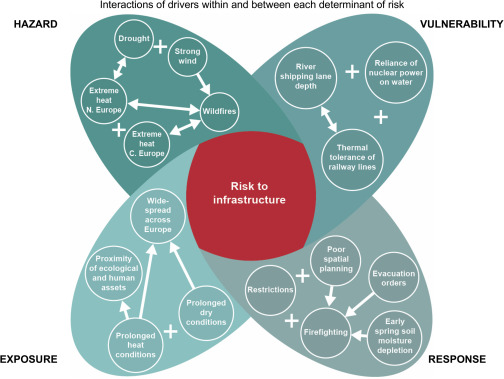
\includegraphics{figures/simpson-risk-framework.jpg}
    \caption{A framework for decomposing risk into its parts: hazard, exposure,
    vulnerability, and response, using risk to infrastructure as an illustrative
    example. Reproduced from Simpson et al. (2021)
    \cite{simpson_framework_2021}.}
    \label{fig:risk-framework}
\end{figure}

\begin{figure}
    \centering
    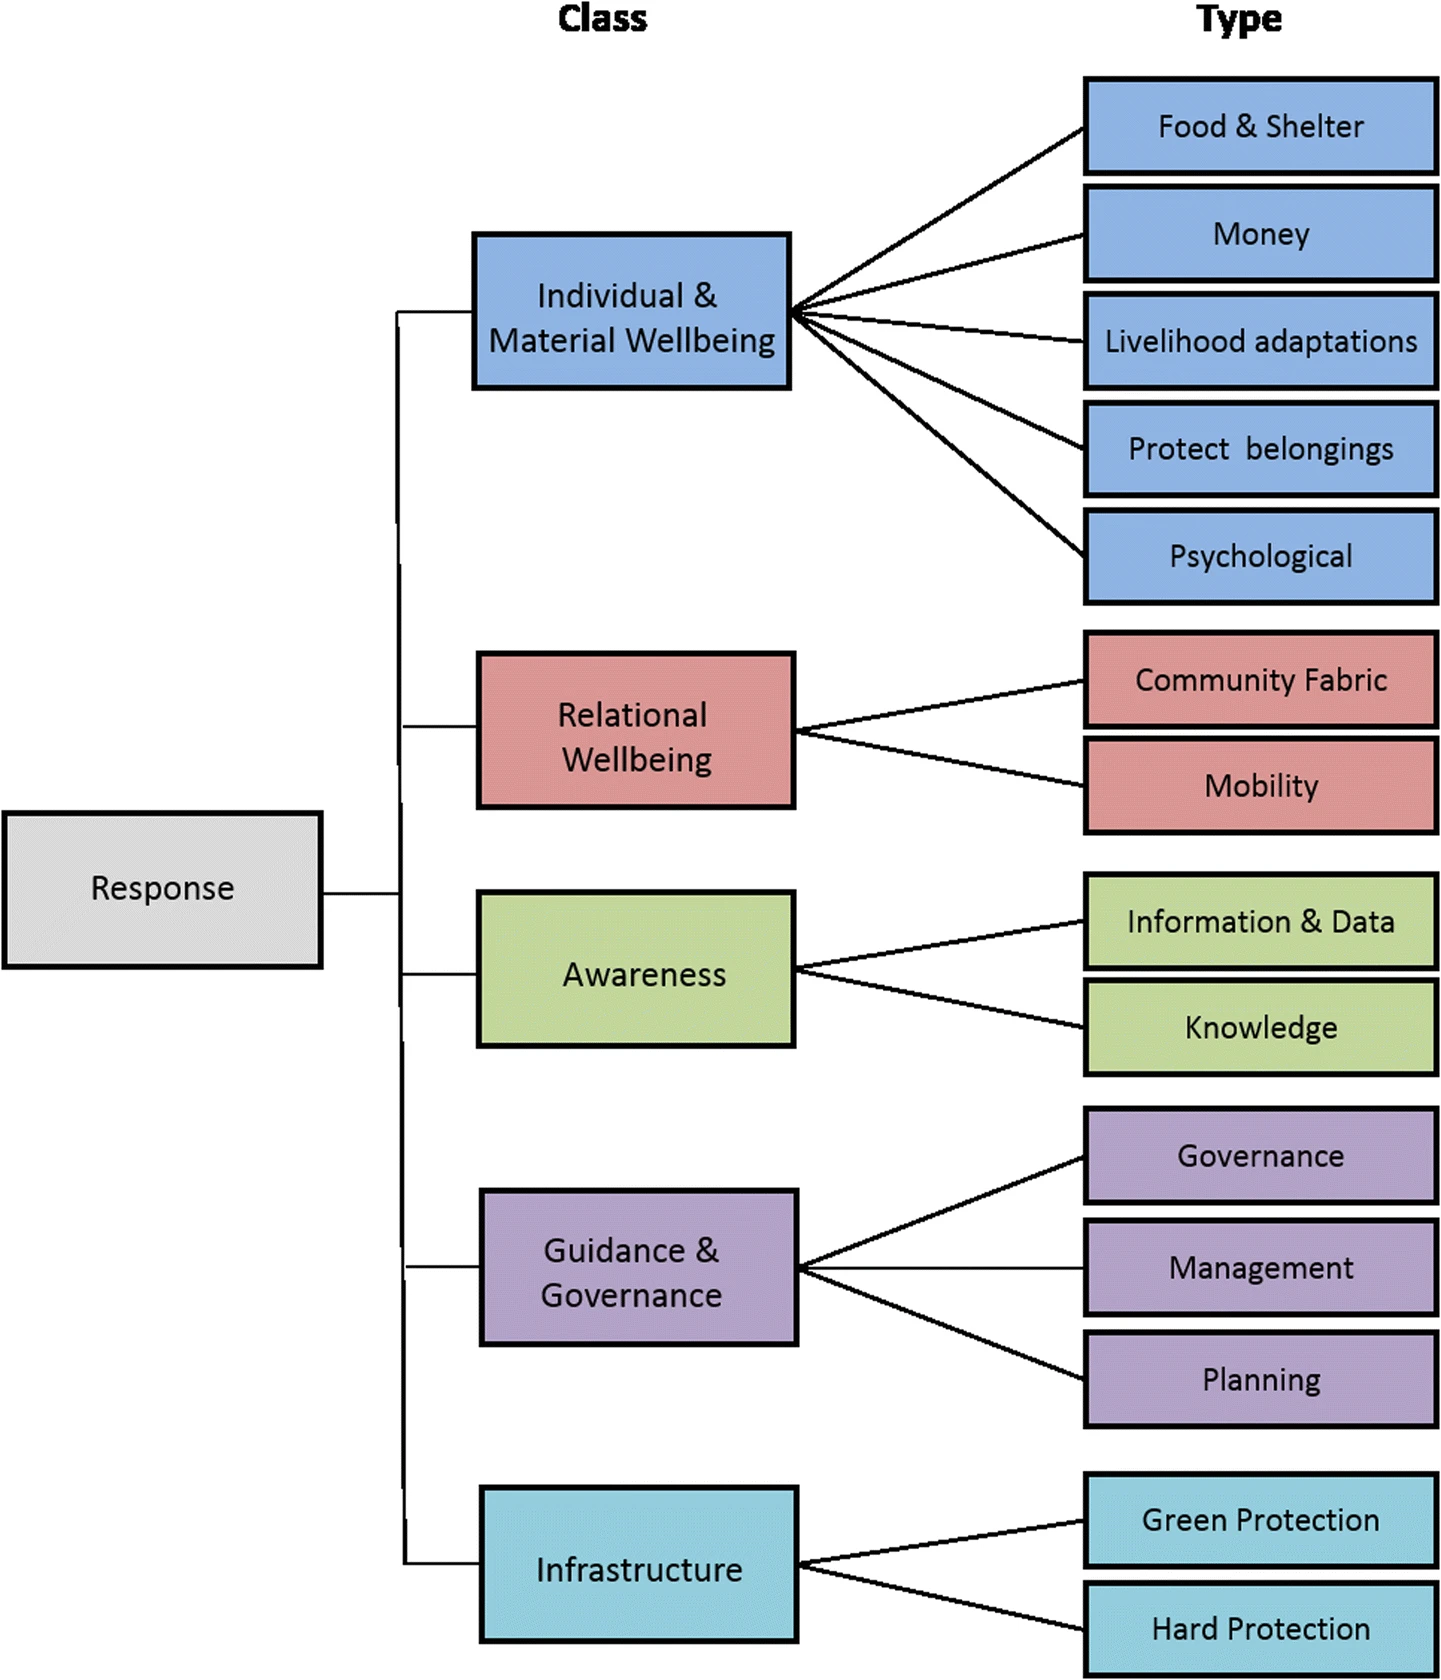
\includegraphics[width=\columnwidth]{figures/risk-response.png}
    \caption{A categorization schema for various responses to climate risks.
    Reproduced from Paterson et al. (2019)
    \cite{paterson_community-based_2019}.}
    \label{fig:risk-response}
\end{figure}

% \noindent\hrulefill \item What are the responses to climate change? How
% successful have climate policies been at achieving climate goals (and
% ultimately achieving net zero carbon emissions)?

Based on the net-zero carbon emissions target set by the 2016 Paris Agreement,
myriad countries, states, and companies have set climate policies covering
two-thirds of the global economy \cite{hale_assessing_2022}. Reducing CO$_2$ (or
CO$_{2eq}$ in some cases) emissions is the primary focus for most of these
policies \cite{fawzy_strategies_2020, roelfsema_taking_2020,
hale_assessing_2022}, which includes the following broad strategies
\cite{fawzy_strategies_2020}:
\begin{enumerate}
    \item Reducing \ac{ghg} emissions by transitioning from fossil-fueled to
    clean energy.
    \item Removing CO$_2$ from the atmosphere using \ac{ccs} and other
    sequestration techniques.
    \item Altering the Earth's energy balance by increasing its albedo and other
    geoengineering concepts.
\end{enumerate}
Despite this, only around five percent of these policies are considered
robust according to their consistency with the \ac{un} ``Race to Zero'' campaign
\cite{hale_assessing_2022}. Further, even the full implementation of national
climate policies leaves approximately  a 28 GtCO$_{2eq}$ gap in \ac{ghg}
emissions \cite{roelfsema_taking_2020}. This gap and the fundamental
assumptions about carbon sequestration from the 2016 Paris Agreement suggest
that the world is on track to overshoot these emissions targets
\cite{roelfsema_taking_2020,taylor_managing_2021}. Carley et al. (2018)
developed a quantitative framework for assessing the vulnerabilities associated
with energy policies or responses \cite{carley_framework_2018}.

% \noindent\hrulefill \item What are the impacts of climate change?

Risk analysis is the first step to a complete understanding of the climate
crisis. The literature on disproportionality further distinguishes
\textit{risks} and \textit{impacts} \cite{dorkenoo_critical_2022}. Consistent
with previous work, a risk is the aggregate of hazards, exposures,
vulnerabilities, and responses. Impacts, then, are the realizations of risk in
terms of loss and damages. This distinction is essential. Responses to
\textit{impacts} are always made \textit{ex post facto}. Differences in
vulnerability to a hazard, often arbitrated by socio-economic status, manifest
as differential impacts. Access to resources conditions an individual's or
community's ability to respond to the impacts of a hazard. Since losses from
impacts disproportionately affect those with the fewest resources, their
vulnerability to future hazards increases in a ``vicious cycle''
\cite{islam_climate_2017, dorkenoo_critical_2022}. In purely economic terms, studies
estimate the 
loss of ecosystem services from land use change associated with climate change
and other human activities at \$4 - \$20 trillion per year (in 2011
\$US) globally, \cite{costanza_changes_2014} and the poorest third of U.S.
counties will experience financial damages between 2 and 20 percent of their
annual income \cite{hsiang_estimating_2017}. However, impacts also have cultural
and psychological dimensions \cite{dorkenoo_critical_2022} that cannot be
captured by accounting for ``externalities.''

% \noindent\hrulefill

% \item How are the damages of climate change distributed, and \textit{why} are
% they distributed this way?

Dorkenoo et al. \cite{dorkenoo_critical_2022} establish \textit{burdens},
injustices arising from social, political, or economic power imbalances, as a
third theme paramount for a holistic understanding of
disproportionality. Burdens influence all aspects of risk and affect access to
resources which condition impacts. Dorkenoo et al. wrote, ``[p]rocesses of
marginalization and exclusion influenced by power struggles [...] influence the
distribution of burdens and consequently responsibilities, in addition to the
different dimensions of climate risk (hazard, exposure, vulnerability [,
response])'' \cite{dorkenoo_critical_2022}. Figure \ref{fig:risk-impact-burden}
demonstrates the mutually reinforcing relationships among risks, impacts, and
burdens. A particularly relevant example of burden is the persistence of energy
burden, where low-income households pay the highest percentage of their income
on energy bills relative to other income groups \cite{brown_high_2020,
cong_unveiling_2022}. Energy burden interferes with electricity access, thereby
increasing vulnerability to extreme heat events \cite{cong_unveiling_2022,
klinenberg_heat_2003}. The risk assessment literature and the energy
system modeling literature typically adopt an apolitical framing of
vulnerabilities. However, inequities do not arise in a vacuum but through
processes of marginalization and exclusion \cite{thomas_explaining_2019}. Often
the distribution of burdens falls along class, race, and gendered lines
\cite{thomas_explaining_2019,mohai_which_2015}. Research on siting patterns of
polluting facilities indicates these projects frequently developed in areas with
people of color and low-income populations \cite{mohai_which_2015}. Pollution
from these facilities creates additional burdens for nearby communities. The
energy justice and environmental justice literature offer insights to contrast this
neutral framing and facilitate normative questions about alternative
distributions \cite{dorkenoo_critical_2022, thomas_explaining_2019}.

\begin{figure}
    \centering
    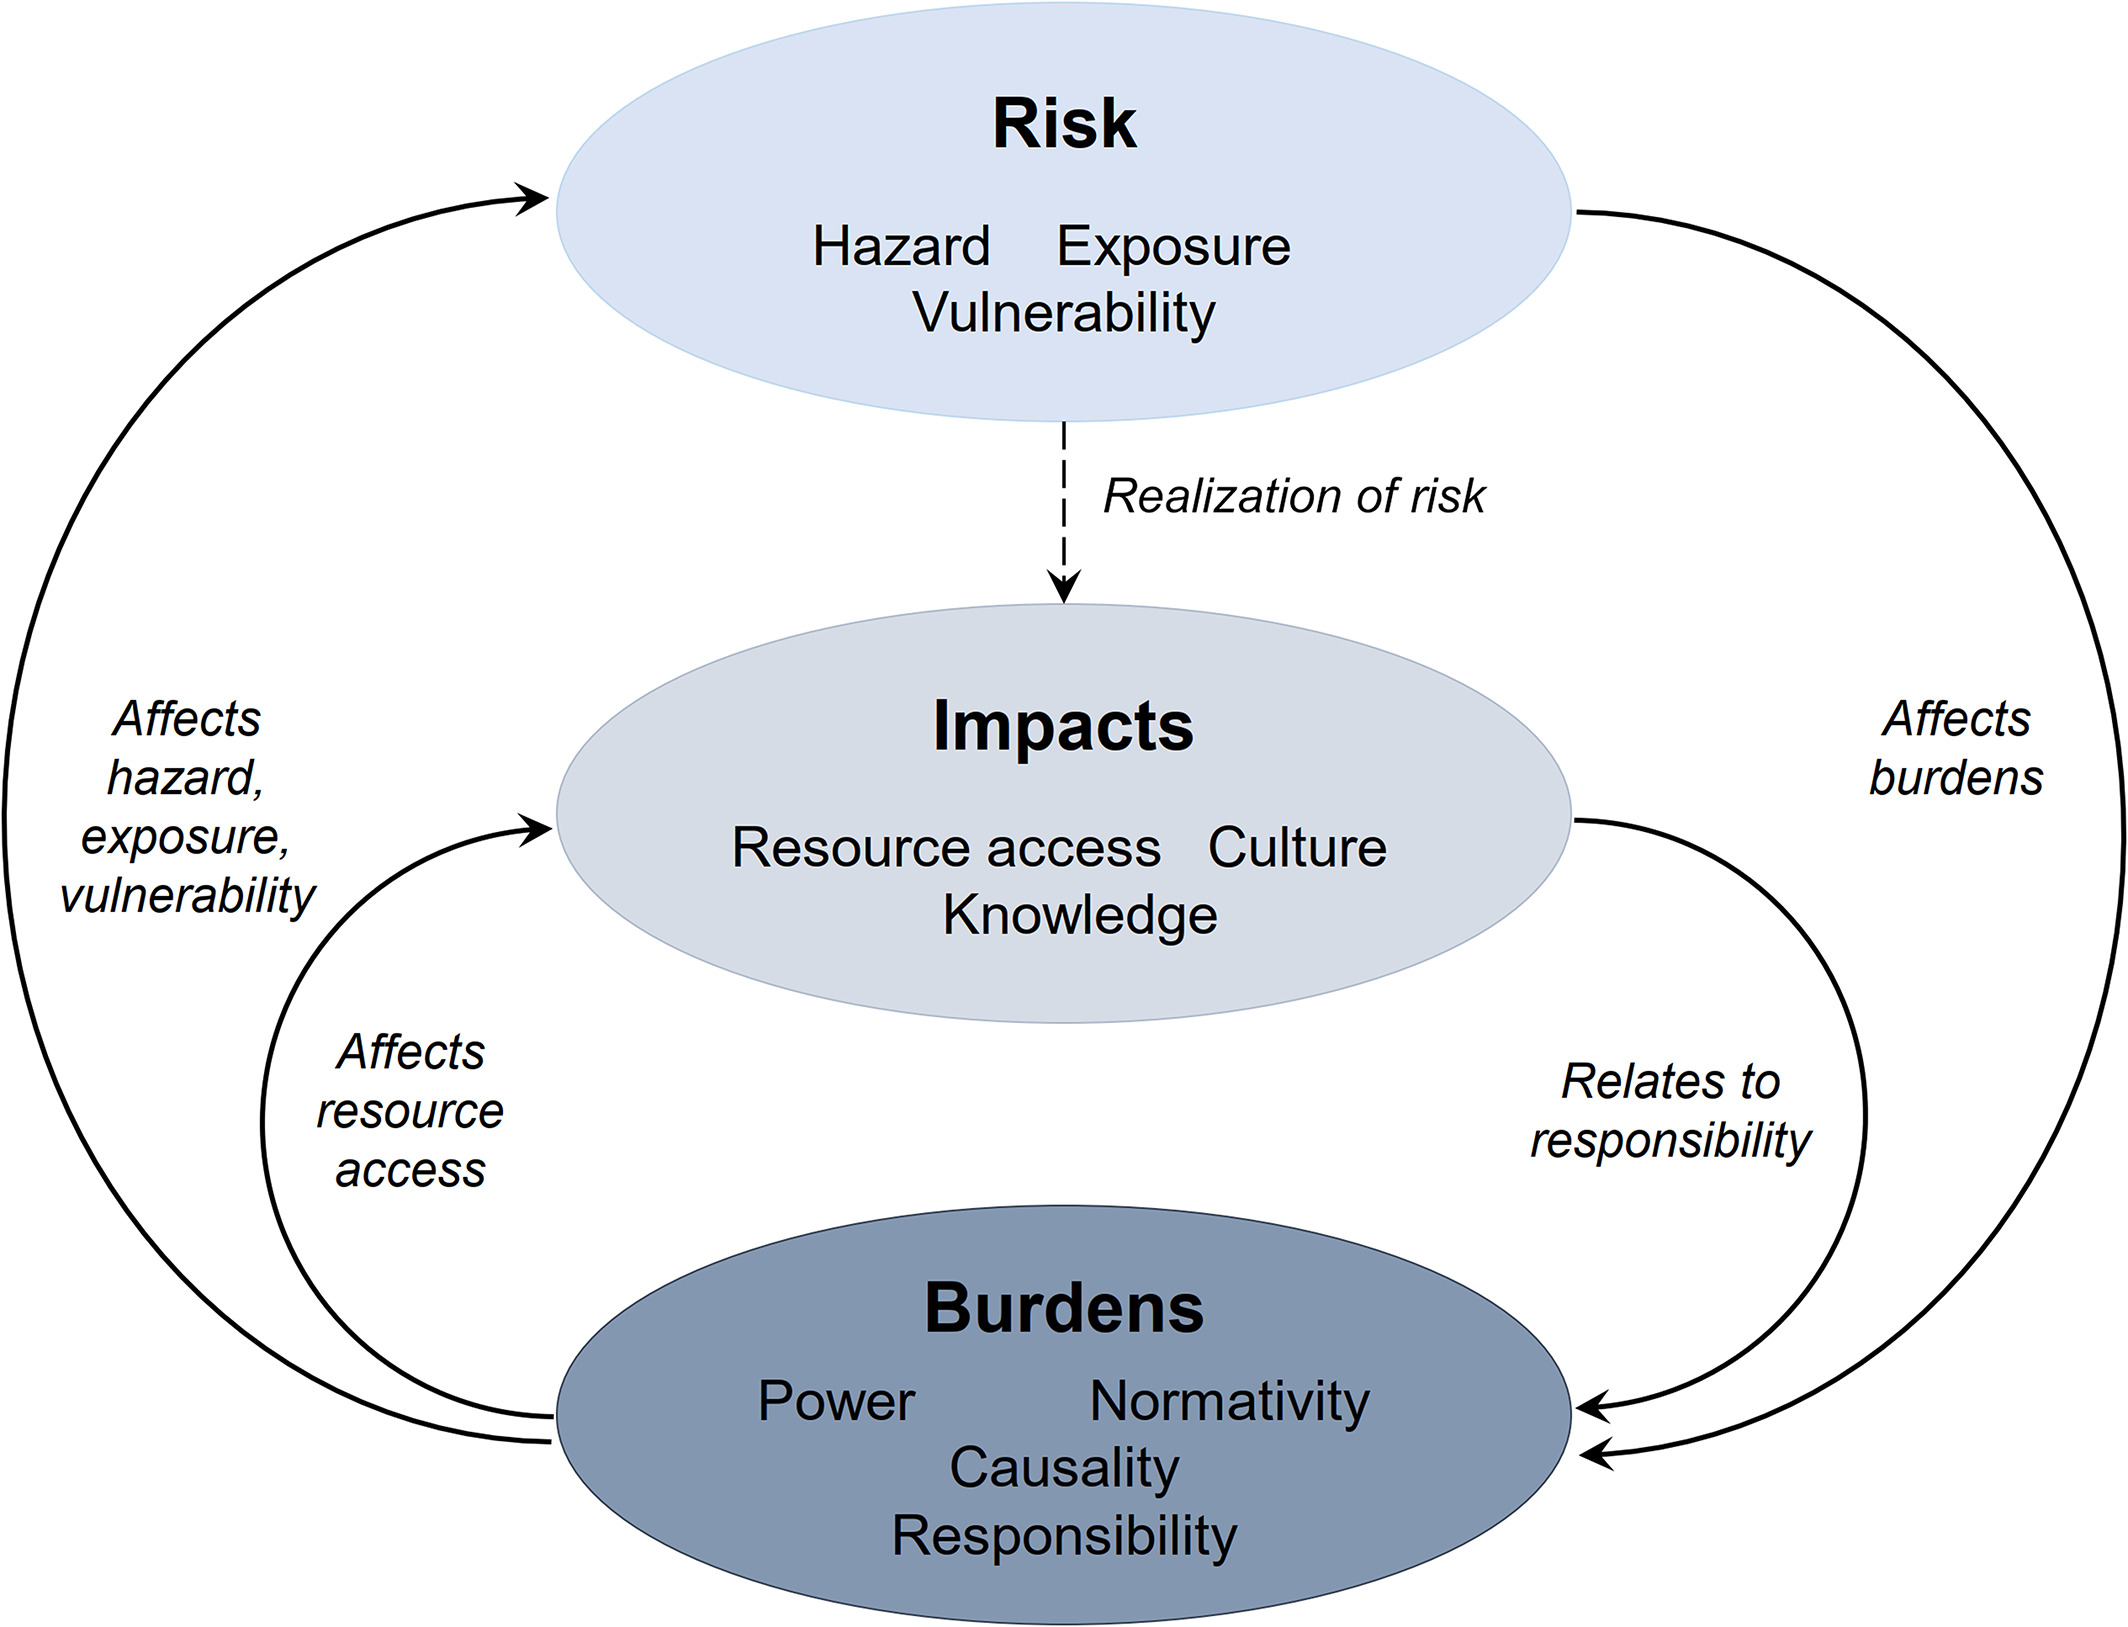
\includegraphics[width=\columnwidth]{figures/dorkenoo-disproportionality.jpg}
    \caption{The relationships among risks, impacts, and burdens. Reproduced
    from Dorkenoo et al. (2022) \cite{dorkenoo_critical_2022}.}
    \label{fig:risk-impact-burden}
\end{figure}


% \noindent\hrulefill

% \textcolor{red}{Subsection: Climate and Energy Systems}
\section{Climate and Energy Systems}

Climate change is driven by \acp{ghg}, a significant byproduct of the
infrastructure that creates, delivers, and consumes energy (i.e., energy
infrastructure). Specifically due to the fraction of carbon emissions already
coming from electricity generation (25 percent in the United States
\cite{us_epa_sources_2020}) and the total decarbonization of the global economy
requiring electrification of other sectors, such as transportation and heat,
thereby increasing the electricity demand, even when accounting for
efficiency improvements
\cite{national_academies_of_sciences_engineering_and_medicine_accelerating_2021,
mai_electrification_2018}, decarbonizing our electricity production is one of
the most critical issues to resolve climate change. Therefore, producing
electricity with zero \acp{ghg} will initiate a cascade of deeper
decarbonization throughout the economy but will require expanded electrical
infrastructure. Accelerating the adoption of clean energy technology is
essential for achieving a stable climate \cite{roelfsema_taking_2020,
taylor_managing_2021}.

% \textcolor{red}{Subsubsection: Technical solutions to energy decarbonization}
\subsection{Technical Solutions to Energy Decarbonization}
% \item What are the technical solutions for decarbonizing the electricity
% sector?

Many studies show that global and local economies can be supported by 100\%
\ac{vre}, such as wind, hydro, and solar power \cite{jacobson_100_2015,
bussar_optimal_2014,brown_response_2018,dorotic_integration_2019,wallsgrove_emerging_2021,
cochran_la100_2021,cosic_100_2012,traber_economically_2021,bogdanov_full_2021,
bogdanov_north-east_2016,
esteban_100_2018,yue_least_2020,neumann_near-optimal_2021}. Yet some countries
that transition to majority \ac{vre} observe higher carbon emissions or a
slower-than-expected reduction due to greater dependence on natural gas
\cite{wagner_co2_2021}. Other studies demonstrate that firm baseload power, such as nuclear power, is
necessary for the deep decarbonization of our energy systems
\cite{wagner_co2_2021,shaner_geophysical_2018,dotson_influence_2022,greene_enhancing_2019,kim_carbon_2021,lehtveer_how_2015,vaillancourt_role_2008,
de_sisternes_value_2016,alzbutas_uncertainty_2012,brook_why_2014,
epiney_economic_2020,petti_future_2018, patrizio_socially_2020}. While some
countries are building new nuclear reactors, and the \ac{nrc} just approved the
first small modular reactor design from NuScale
\cite{office_of_nuclear_energy_science_and_technology_nrc_2023}, other places
are shutting down their operating nuclear plants \cite{johnson_new_2021}. 
% In the latter cases, places that shut down nuclear plants always saw a subsequent rise
% in carbon emissions due to greater dependence on natural gas.
% \textcolor{red}{Show plot of carbon emissions vs time for New York?}. 
Further,
the only examples of highly decarbonized electrical grids are places with a high
penetration of hydro or nuclear power and the former is widely considered
exhausted. There is nearly universal agreement that decarbonizing electricity
requires phasing out fossil-fueled power plants and a significant expansion of
clean electricity generators. Although many studies show the
\textit{feasibility} of a variety of energy mixes, the following is strongly
debated in the literature.
\begin{enumerate}
    \item Whether energy systems should be 100\% renewable or if nuclear power and
    \ac{ccs} should be included \cite{heard_burden_2017,
    brown_response_2018,elmallah_frontlining_2022, brook_why_2014}.
    \item What the role of distributed and decentralized energy sources in
    expanding our energy infrastructure should be
    \cite{pitt_assessing_2015,rinaldi_what_2022,parag_electricity_2016,wang_modeling_2020,
    morvaj_decarbonizing_2017,gilbert_can_2020,li_economic_2016,falke_multi-objective_2016}.
\end{enumerate}
The strength of the technical arguments on both sides of these discussions
combined with the distinct lack of sufficient policy agendas pursuing any of
them \cite{roelfsema_taking_2020,hale_assessing_2022}, suggests the existence of
poorly articulated trade-offs and that technical solutions cannot be assessed
from an engineering perspective, alone. Some researchers and policymakers
disagree on technical grounds, while others disagree on the basis of
institutional or systemic injustices. There are also differences in values. Indeed, the cultural theory of risk argues that our social constructions, rather than risks themselves, dictate what threats are recognized and their 
corresponding liabilities and benefits \cite{mcneeley_cultural_2014, van_de_graaff_understanding_2016}.
Clean technologies like nuclear power and renewables, such as solar or wind
power, are not only different in how they produce electricity but also in the
values and paradigms they represent. Sometimes, communication fails because the
question being discussed is not agreed upon either. Often, feasibility studies
address the positivist question, ``what is the least-cost pathway to the energy
transition,'' while others consider more normative questions, such as ``how
should we proceed equitably?'' Normative questions are qualitative and,
therefore, inherently challenging to answer and require the application of
ethics. Indeed there are many more normative questions than positive ones.
\textcolor{black}{Is perfect the enemy of good? How do we balance stakeholder
preferences, upstream and downstream effects, and the necessity to respond
quickly to climate change? Will this mix of influences lead to paralysis or
inaction?} \textcolor{black}{Given climate change's complex, interacting, and
disproportionate nature, engineering alone is ill-equipped to resolve the
problem. Ideas from the environmental and energy justice literature offer a
social perspective for addressing the risks and impacts of climate change
hazards.}
% \noindent\hrulefill \textcolor{red}{Subsubsection: Energy justice and the
% Boundaries of Energy Systems.}
\subsection{Energy Justice}

% \item What is energy justice?


Energy justice is a conceptual and analytical tool regarding the ethical or
normative dimensions of energy systems and addresses the systemic causes of
burdens, and inequities \cite{sovacool_energy_2015}. 

% \begin{enumerate} \item What is justice?
    
    There are many conceptions of justice; however, the most popular framework
    for understanding justice is a three-faceted approach originating from David
    Schlosberg: distributional, recognitional, and procedural justice
    \cite{schlosberg_2_2007}.
    % \item What is distributional justice? 
% \noindent\hrulefill
    Distributional justice relates to the fair distribution of resources,
    burdens, and responsibilities. Studies on distributional justice seek to
    address the normative question: how should a just society distribute the
    benefits it produces and \textit{the burdens required to maintain it}
    \cite{brighouse_justice_2004}. Additionally, distributional justice
    considers \textit{how} poor distributions are created
    \cite{schlosberg_2_2007}.
% \noindent\hrulefill
    % \item What is procedural justice?
    Procedural (in)justice is defined as the presence of (un)fair and
    (in)equitable institutional processes of the state \cite{schlosberg_2_2007}.
    In other words, how decisions of societal import are made and who is
    involved in those decisions. Sovacool and Dworkin (2015) outline four
    elements of procedural justice: transparency, meaningful participation,
    impartiality, and avenues for redress \cite{sovacool_energy_2015}.    
% \noindent\hrulefill
    % \item What is recognition justice?
Justice of recognition is the vaguest of the three tenets of justice and is
    frequently reduced to a component of either distribution or procedural
    justice \cite{schlosberg_2_2007, van_uffelen_revisiting_2022}. A common
    argument for this consolidation is that recognition is a precondition for
    achieving distributional justice or that achieving procedural justice
    necessarily includes recognition \cite{schlosberg_2_2007}. However,
    recognition is unique from distributive and procedural justices because it
    is concerned with a different family of injustice, namely,
    \textit{misrecognition} \cite{van_uffelen_revisiting_2022}. van Uffelen
    (2022) suggests a nuanced definition of recognition justice as ``the
    adequate recognition of all actors through love, law, and the status order''
    \cite{van_uffelen_revisiting_2022}.
% \end{enumerate} \noindent\hrulefill
Sovacool and Dworkin (2015) offer a framework for assessing energy policies from
a justice perspective. Table \ref{tab:justice-frameworks} map the relationships
between justice-as-a-decision-making-tool from Sovacool \& Dworkin, Paterson's
hazard response characterization, and Schlosberg's triumvirate of justice. 

\begin{table}[h]
    \centering
    \caption{Different ways to operationalize justice concepts.}
    \begin{tabular}{ccc}
    \toprule
    Schlosberg \cite{schlosberg_2_2007} & Sovacool \& Dworkin 
    \cite{sovacool_energy_2015}& Paterson et al. \cite{paterson_community-based_2019}\\
    \midrule
    & Intragenerational Equity & Material Well-being \\
    Distribution & Intergenerational Equity & Infrastructure \\
    & Responsibility & \\
    & Due Process & Awareness \\
    Procedure & Good Governance & Governance \\
    & & \\
    & Availability$^1$ & Relational Well-being \\
    Recognition & Affordability$^1$ & \\
    & Sustainability$^1$ & \\
    \bottomrule\\
    % \rule{0pt}{2ex}
    \multicolumn{3}{l}{$^1$ van Uffelen \cite{van_uffelen_revisiting_2022} argues for this categorization.}
\end{tabular}
    \label{tab:justice-frameworks}
\end{table}

Although Sovacool \& Dworkin do not explicitly discuss recognition justice, it
is a unique aspect of justice that can still be useful for contextualizing their
recommendations. For example, due to the psychological pressures introduced by a
lack of access to energy, either due to infrastructure or cost, interrupts
relational well-being and is an injustice \cite{van_uffelen_revisiting_2022}.
Further, (un)sustainable policies may be considered a misrecognition of the
humanity of future generations.

\textcolor{black}{Next, I examine the specific ways the social science literature understands how energy systems and their infrastructure (artifacts) contribute to the distribution of burdens.}

% \noindent\hrulefill \item What is an energy system?
\subsection{Boundaries of Energy Systems}
\label{section:energy-system-boundaries}
Previous work defined energy systems in purely technical terms as spatially,
temporally, and topologically complex machines that coordinate the supply and
demand of energy, especially electricity \cite{dotson_influence_2022}. However,
this definition neglects the ways energy systems may be used to construct and
maintain power relations that contribute to inequitable distributions of
burdens. Energy access is necessary to support complex modern economies and
therefore possesses political power \cite{jones_building_2013,
bridge_energy_2018}. The literature on the political economy of energy
infrastructure locates this political influence in five distinct ways
\cite{bridge_energy_2018}. First, energy infrastructure affects competition and
collaboration among nation-states in the geo-political sphere. The current
situation in Ukraine makes this especially salient
\cite{figueiredo_impacts_2022}. 

The second subset of the literature focuses on the process of energy
infrastructure development and how these processes create social inequities. For
example, energy policies that subsidize residential solar panels have not led to
more equitable adoption of solar energy, with greater adoption in areas with
higher income, among other social indicators \cite{reames_distributional_2020}.
Other popular arguments in favor of renewable energy assert that these energy
sources are necessarily more egalitarian because the Sun and the wind cannot be
(or have not yet been) privatized. Another is the urgency of climate change.
While true, ignores or minimizes the potential environmental and social
consequences of energy planning that does not consider energy justice
\cite{jones_building_2013}. Large-scale energy projects in the Global South have
already led to the dispossession of nearby indigenous communities and other key
actors \cite{yenneti_spatial_2016, barragan-contreras_procedural_2022}.

Third, the development of energy infrastructure is not simply conducted via
policy measures, but also in the manner governments activate the public
imagination in favor of these policies
\cite{bridge_energy_2018,jasanoff_containing_2009}. Jasanoff and Kim (2009)
articulate this concept as `socio-technical imaginaries,' which are
simultaneously descriptive and prescriptive of possible energy futures
established by governments in the national zeitgeist
\cite{jasanoff_containing_2009}. This concept is demonstrated by the discourse
surrounding nuclear energy in the United States and South Korea
\cite{jasanoff_containing_2009} as well as in Japan
\cite{valentine_energy_2019}. Governments can employ `grand narratives' related
to national security, climate change, or modernization to enhance public support
while minimizing genuine participation \cite{bridge_energy_2018}.

Fourth, the political power of energy infrastructure can be traced further to
the cultural values and policy choices embedded in the design and operation of
seemingly technical systems \cite{bridge_energy_2018}. In other words, the
design and implementation of energy infrastructure may be used as a vehicle for
apparently unrelated agendas, a form of ``policy-making by other means''
\cite{bridge_energy_2018, clausewitz_chapter_1918}. Edwards and Hecht (2010)
refer to the co-constitution of technological and political order as
`\textit{technopolitics},' demonstrating the tangible material and political
outcomes of technological systems \cite{edwards_history_2010}.

Finally, energy systems and their infrastructure possess a unifying quality
through which new political identities may evolve \cite{bridge_energy_2018}.

From these various perspectives, we can observe that confining an energy system
to its technical characteristics is woefully incomplete. I propose that an
energy system is a spatially, temporally, and topologically complex machine that
coordinates the supply and demand of energy and acts as an important mediator of
burdens that influence climate change risk. This thesis takes the important step
of analyzing energy system planning and policy with this expanded definition.

% \textcolor{red}{Climate change \textit{is} a complex issue with multiple
% interacting and interwoven layers. However, it can and must be understood
% holistically instead of stripping it of its complexity and exclusively
% relegating solutions to the realms of economics and engineering. This
% over-simplification is done out of a misplaced sense of pragmatism and either an
% inability or unwillingness to completely apprehend the problem.}

% \noindent\hrulefill
% \item What are the obstacles to building more clean energy infrastructure?
% What is preventing the transition to a ``qualitatively new type of
% [environmental] society'' \cite{bluhdorn_legitimation_2020}?

% \textcolor{red}{This is where you can introduce different schools of thought
% about transitions.}

% \textcolor{blue}{Interesting that you chose to frame public acceptance as an
% ``obstacle'' rather than a source of greater accountability and
% participation.} \begin{enumerate} \item Legitimation crisis of democracy
% \cite{bluhdorn_legitimation_2020}. \item Social acceptance literature
% \end{enumerate}

% \end{enumerate}

% \section{Calls for a Just-Transition}

% Att

The next section reviews current attempts to model energy systems and identifies
gaps in conventional methods.
